\subsubsection{Test}
%Det indkøbte kamera er testet ved at tage en serie af billeder af langerhanske øer. Billedserien skulle i første omgang danne grundlag for den videre billedbehandling. Første test bestod af 107 billeder taget af langerhanske øer, herunder billeder kun af isolerede øer og enkelte baggrundsbilleder. Forsøgsopstillingen var en efterligning af den nuværende sorteringsproces, hvor opløsningen hældes i petriskåle. Petriskålen placeres på en sort bagplade, hvorefter operatøren isolerer øerne ved at kigge gennem et mikroskop. Forsøgsopstillingen er vist i figur \ref{fig:kameraopstillingen}. 
%\begin{figure}[H]
%	\centering
%	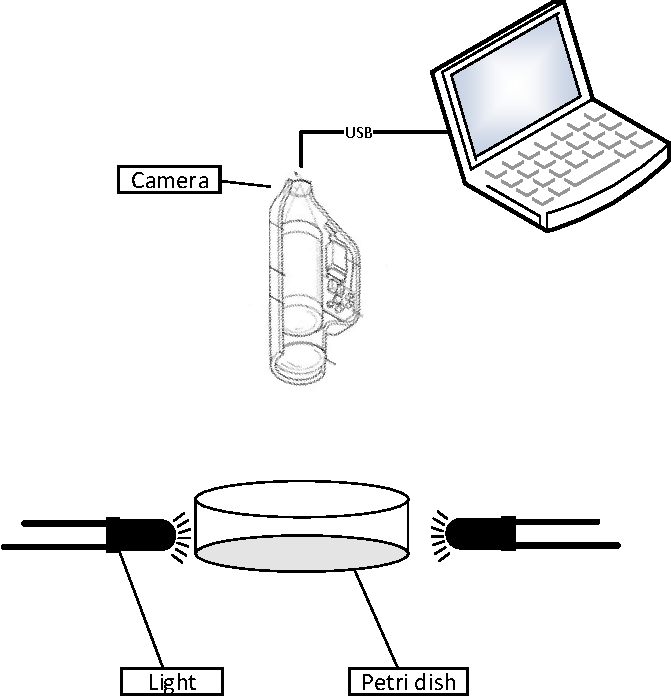
\includegraphics[width=0.6\textwidth]{billeder/software/kameraopstil-crop.pdf}
%	\caption{Forsøgsopstilling}
%	\label{fig:kameraopstillingen}
%\end{figure}
I forsøgsopstillingen anvendtes der i stedet for mikroskopet det indkøbte kamera. En række billeder blev udvalgt til yderligere analyse, hvor Søren Gregersen udpegede hvilke elementer der var øer. På billede \ref{fig:isletSG} er der markeret, hvor en ø er placeret.

\begin{figure}[H]
	\centering
	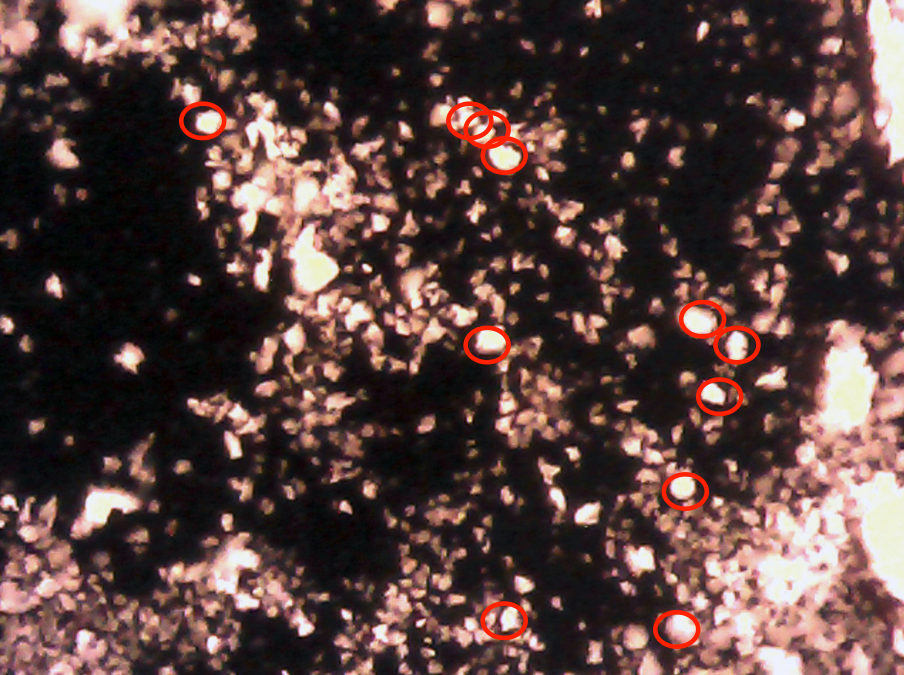
\includegraphics[width=0.6\textwidth]{billeder/software/sgbillede.png}
	\caption{Øer udpeget af Søren Gregersen}
	\label{fig:isletSG}
\end{figure}

Efter nærmere analyse af billederne viste det sig at det indkøbte kamera ikke var tilstrækkelig kvalitet til at lave segmentering på billederne. Når øerne blev observeret gennem et almindeligt mikroskop var der langt større kontrast i mellem øerne og det ekstra væv. På billederne fra kameraet er der ikke denne forskel, hvilket udelukker segmentering på denne parameter. Det kan ses på billede \ref{fig:isletSG} at der er områder hvor lysintensiteten er lige så høj, som de steder hvor øerne er markeret. Dette gør, at segmentering på baggrund af lysintensiteten kan udelukkes. Herudover er det tydeligt, at billederne ikke er skarpe nok, hvilket gør at det er svært at vurdere hvad der er øer og ikke øer. De parametre, hvor kameraets kvalitet ikke er tilstrækkelig er derfor bl.a. autoeksponering og autofokus. En bedre styring af autoeksponeringen ville kunne give et bedre kontrast forhold i mellem øerne og det omkringliggende væv, mens en bedre autofokus ville hjælpe på skarpheden i billedet, hvilket muliggøre segmentering baseret på strukturer.

Herudover er der er en polariserende effekt på billederne, hvor nogle af elementerne lyser meget kraftigt op grundet belysningen. Dette gør det er svært at vurdere strukturer og størrelser på elementerne i billedet. 

Efter den første test blev det i samarbejde med vejleder og kunde besluttet, at det indkøbte kamera ikke er af tilstrækkelig kvalitet til at detektere langerhanske øer. I dette system bliver der i stedet udviklet et sæt af billeder, som skal simulerer flowet i slangerne. Billederne skal indeholde langerhanske øer, ekstra væv og tilfældig støj for at få dem til at ligne tæt på det man observerer gennem et almindeligt mikroskop. Udfra disse billeder skal langerhanske øer detekteres, hvorefter systemet skal åbne ventilen. Billedesættet skal ses som en simulering af kameraet. I en senere prototype vil et kamera af højere kvalitet være påkrævet. Her er det især krav til bedre autoeksponering og autofokus som er essentielle. Dette vil være nødvendigt for at øge kontrasten i mellem øerne og det omkringliggende væv for bedre segmentering. Herudover vil et kamera med polariseringsfilter være en mulighed til at fjerne evt. genskær fra belysningen. Hos Farnell er der andre producenter end det indkøbte Duratool mikroskop, som bl.a. har polariseringsfilter. En test af forskellige kameraer ville være oplagt til finde det ideelle kamera til optagelse af langerhanske øer. 